\documentclass[fleqn, 11pt]{article}

\usepackage{verbatim}
\usepackage{amsmath}
\usepackage{amssymb}
\usepackage{amsthm}
\usepackage{hyperref}
\usepackage{ulem}
\usepackage{enumitem}
\usepackage[top=1.0in, left=0.75in, right=0.75in, bottom=0.75in]{geometry}
\usepackage{graphicx}
\usepackage{subcaption}

\newcommand{\myline}{
    \par
    \kern3pt % space above the rules
    \hrule height 0.5pt
    \kern2pt % space between the rules
    \hrule height 0.5pt
    \kern3pt % space below the rules
    \par
}

\usepackage[T1]{fontenc}

\newcommand{\bs}[1]{\boldsymbol{#1}}
\newcommand\norm[1]{\left\lVert#1\right\rVert}

\usepackage{array}
\usepackage{caption}
\usepackage{floatrow}
\usepackage{multirow}

\usepackage{chngcntr}
\counterwithin*{equation}{section}

\usepackage{sectsty}
\sectionfont{\centering}

\usepackage[perpage]{footmisc}

\usepackage{fancyhdr}
\pagestyle{fancy}
\fancyhf{}
\lhead{190100036 \& 190100044}
\rhead{SI424: Project}
\renewcommand{\footrulewidth}{1.0pt}
\cfoot{Page \thepage}

\setlength{\parindent}{0em}
\renewcommand{\arraystretch}{2}%

\title{SI424: Statistical Inference \\ Project Report}
\author{
    \begin{tabular}{|c|c|}
        \hline
        \textsf{Krushnakant Bhattad} & \textsf{ \hspace{5pt} Devansh Jain \hspace{5pt} } \\
        \hline
        \textsf{190100036} & \textsf{190100044}\\
        \hline
    \end{tabular}
}
\date{Autumn 2021}

\begin{document}

\maketitle
\thispagestyle{empty}
\renewcommand{\arraystretch}{1}%
\setcounter{page}{0}

\myline
\vspace{10pt}
\underline{\large {\textsc{Project Title}}}:

\medskip

Experiments on Parameter Estimation and Hypothesis Testing

\vspace{7pt}
\myline
\vspace{10pt}
\underline{\large {\textsc{Abstract}}}:

\medskip

We first devise two problems on parameter estimation. We perform experiments for different sample size and observe the varied value of estimates.

We also devise two problems on hypothesis testing. We perform experiments for different sample size and different true values and observe the variation in Type I error and Type II error.

\vspace{7pt}
\myline
\vspace{10pt}
\underline{\large {\textsc{Associated GitHub Repository}}}:

\medskip

The GitHub repository can accessed at: \url{https://github.com/devansh-dvj/SI424-Project}

\vspace{7pt}
\myline
\vspace{10pt}
\underline{\large {\textsc{Common Notations}}}:

\medskip

$\mathcal{N}(\mu, \sigma^2)$ denotes the Normal distribution with mean $\mu$ and variance $\sigma^2$. \\
$\mathrm{Binomial}(p, n)$ denotes the Binomial distribution with probability of success $p$ and number of trials $n$. \\
$\mathrm{Uniform}[\theta_1, \theta_2]$ denotes the Uniform distribution with lower bound $\theta_1$ and upper bound $\theta_2$. \\
$\mathrm{mean}(x)$ denotes mean of elements in vector $x$. \\
$\mathrm{max}(x)$ denotes maximum of elements in vector $x$. \\
$\mathrm{min}(x)$ denotes minimum of elements in vector $x$.

\vspace{7pt}
\myline


\newpage
\section{Parameter estimation Problem 1}
\setcounter{figure}{0}
\subsection{Description}
The population growth rate of Italy follows $\mathcal{N}(\mu, \sigma^2)$ distribution. \\
We have population growth rate $g = (g_1, \cdots ,g_n)$ of different years given to us for Italy. \\
Estimated values are $\hat{\mu}_{MLE} = \mathrm{mean}(g)$ and $\hat{\sigma}_{MLE} = \sqrt{ \mathrm{mean}((g - \hat{\mu}_{MLE})^2) }$.

\subsection{Experiment}
From \verb!population_Country.csv!, we determine population growth rate for Italy. \\
The population growth rates are computed as percentage change in population (using \verb!Total2! column) for every year. \\
The size of the list is 147 for Italy. \\
We randomly choose a $K$ sized subset $(K \le 147)$ of the list (i.e. take a $K$-sized sample). We compute the estimate of $\mu$ and $\sigma$ ($\hat{\mu}_{MLE}$ and $\hat{\sigma}_{MLE}$) using this sample. We repeat this for $N$ iterations. Basically, we carry out $N$ experiments of estimation on $K$ sized sample. \\
We intend to observe the variation in our estimate of $\mu$ and $\sigma$ for different $K$ and $N$.

\subsection{Results}
\subsubsection{Estimate of $\mu$}
\begin{figure}[H]
    \centering
    \begin{subfigure}[H]{0.49\textwidth}
        \centering
        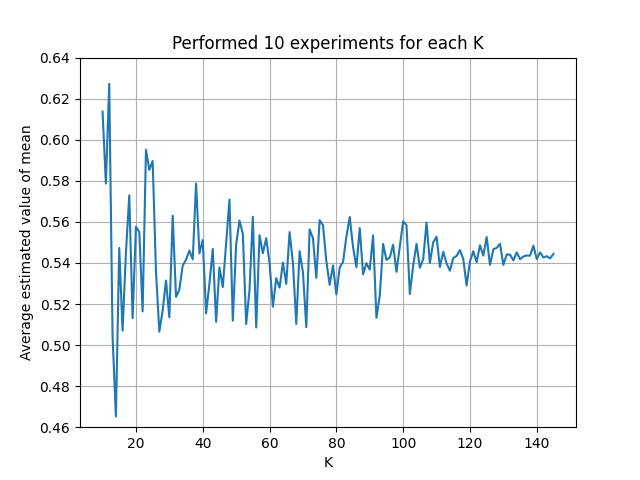
\includegraphics[width=\textwidth]{P1_mu/avgs_10.png}
        \caption[]{Average value of $\hat{\mu}_{MLE}$ observed}
    \end{subfigure}
    \begin{subfigure}[H]{0.49\textwidth}
        \centering
        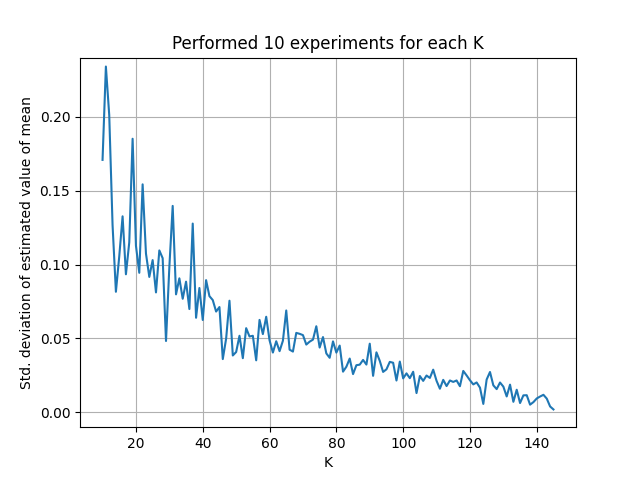
\includegraphics[width=\textwidth]{P1_mu/stds_10.png}
        \caption[]{Std. deviation of $\hat{\mu}_{MLE}$ observed}
    \end{subfigure}
    \caption{Number of iterations, $N = 10$}
\end{figure}
\newpage
\begin{figure}[H]
    \centering
    \begin{subfigure}[H]{0.49\textwidth}
        \centering`
        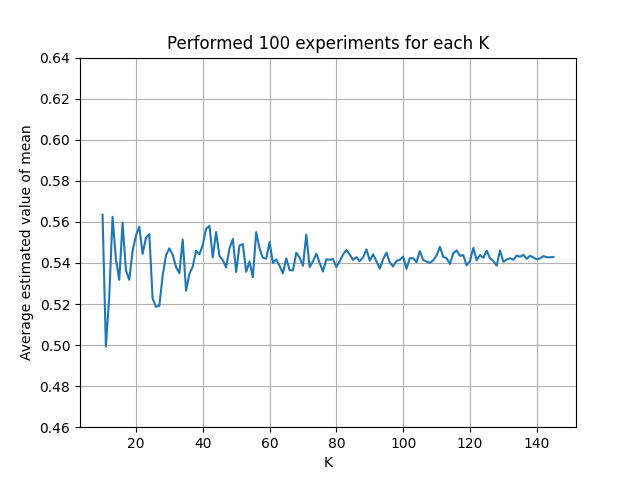
\includegraphics[width=\textwidth]{P1_mu/avgs_100.png}
        \caption[]{Average value of $\hat{\mu}_{MLE}$ observed}
    \end{subfigure}
    \begin{subfigure}[H]{0.49\textwidth}
        \centering
        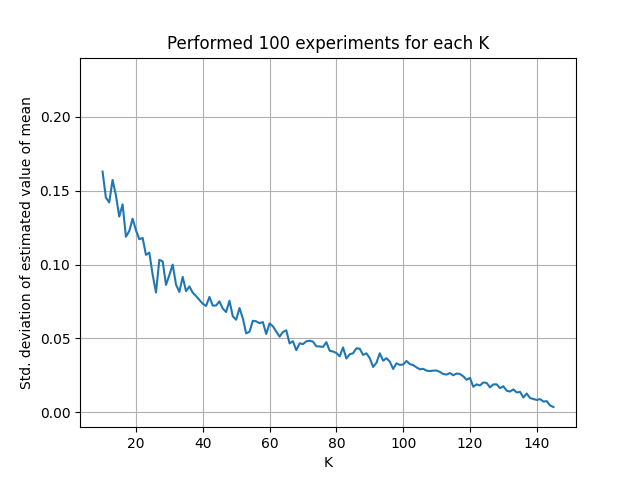
\includegraphics[width=\textwidth]{P1_mu/stds_100.png}
        \caption[]{Std. deviation of $\hat{\mu}_{MLE}$ observed}
    \end{subfigure}
    \caption{Number of iterations, $N = 100$}
\end{figure}
\vspace{30pt}
\begin{figure}[H]
    \centering
    \begin{subfigure}[H]{0.49\textwidth}
        \centering
        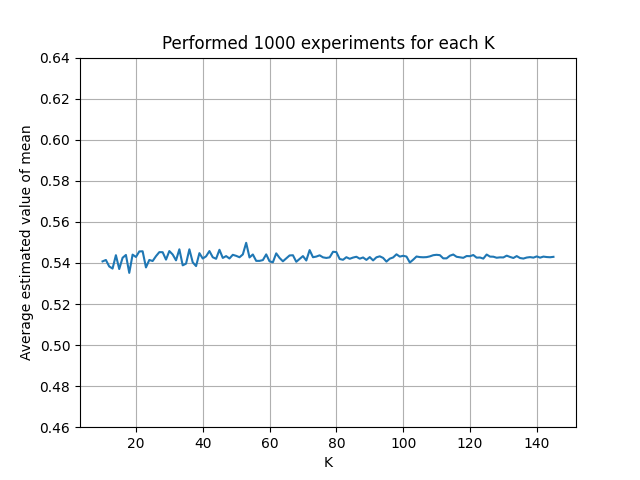
\includegraphics[width=\textwidth]{P1_mu/avgs_1000.png}
        \caption[]{Average value of $\hat{\mu}_{MLE}$ observed}
    \end{subfigure}
    \begin{subfigure}[H]{0.49\textwidth}
        \centering
        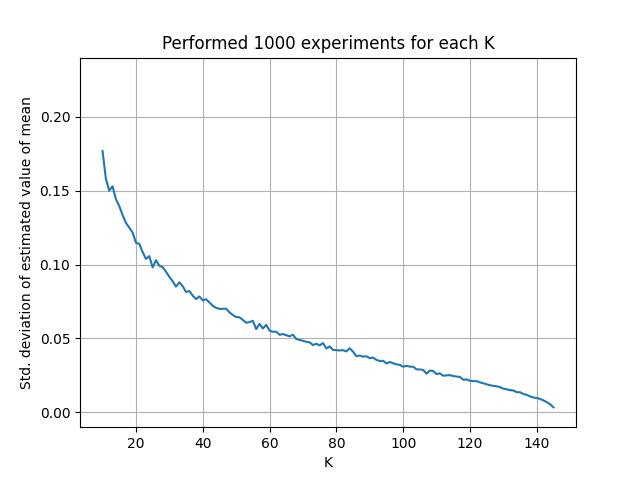
\includegraphics[width=\textwidth]{P1_mu/stds_1000.png}
        \caption[]{Std. deviation of $\hat{\mu}_{MLE}$ observed}
    \end{subfigure}
    \caption{Number of iterations, $N = 1000$}
\end{figure}
\newpage
\subsubsection{Estimate of $\sigma$}
\begin{figure}[H]
    \centering
    \begin{subfigure}[H]{0.49\textwidth}
        \centering
        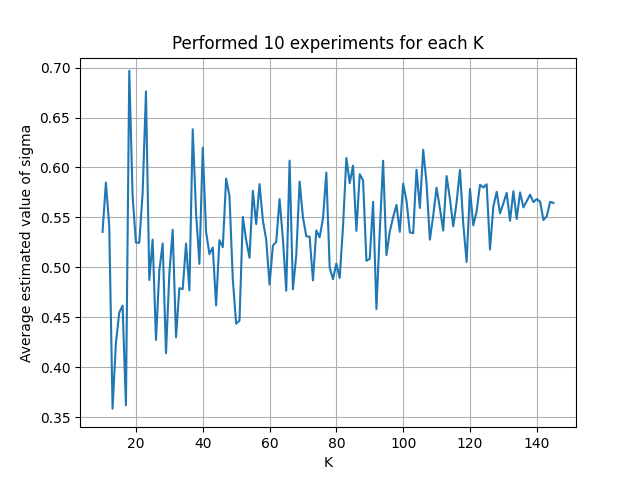
\includegraphics[width=\textwidth]{P1_sigma/avgs_10.png}
        \caption[]{Average value of $\hat{\sigma}_{MLE}$ observed}
    \end{subfigure}
    \begin{subfigure}[H]{0.49\textwidth}
        \centering
        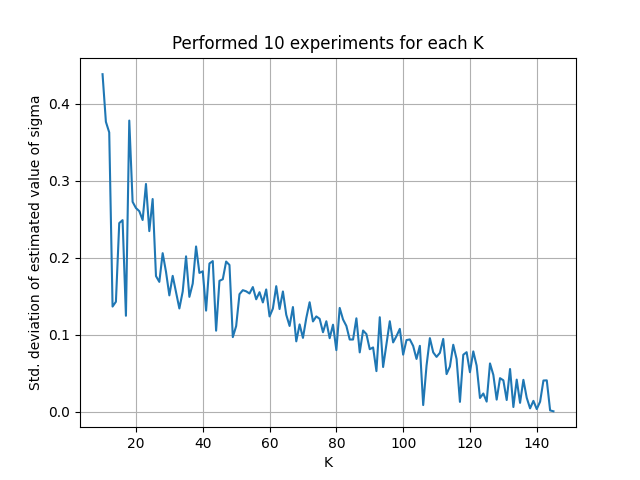
\includegraphics[width=\textwidth]{P1_sigma/stds_10.png}
        \caption[]{Std. deviation of $\hat{\sigma}_{MLE}$ observed}
    \end{subfigure}
    \caption{Number of iterations, $N = 10$}
\end{figure}
\vspace{30pt}
\begin{figure}[H]
    \centering
    \begin{subfigure}[H]{0.49\textwidth}
        \centering
        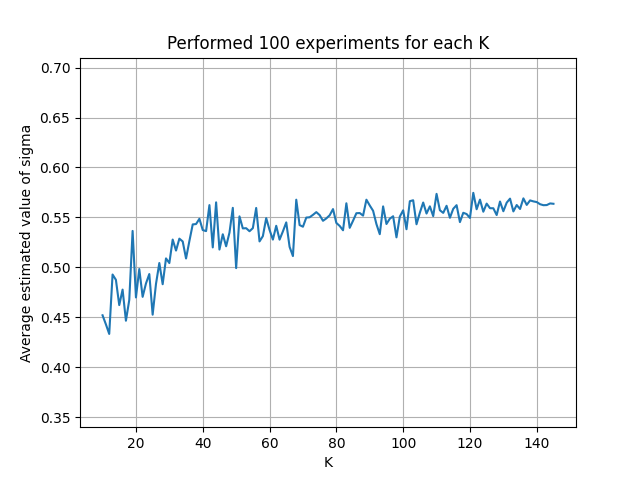
\includegraphics[width=\textwidth]{P1_sigma/avgs_100.png}
        \caption[]{Average value of $\hat{\sigma}_{MLE}$ observed}
    \end{subfigure}
    \begin{subfigure}[H]{0.49\textwidth}
        \centering
        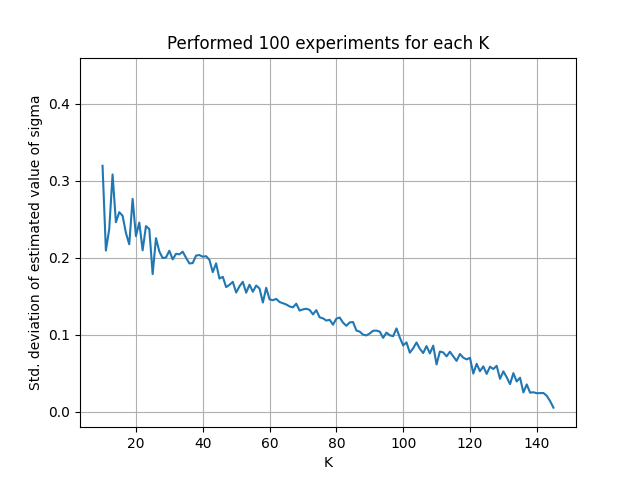
\includegraphics[width=\textwidth]{P1_sigma/stds_100.png}
        \caption[]{Std. deviation of $\hat{\sigma}_{MLE}$ observed}
    \end{subfigure}
    \caption{Number of iterations, $N = 100$}
\end{figure}
\newpage
\begin{figure}[H]
    \centering
    \begin{subfigure}[H]{0.49\textwidth}
        \centering
        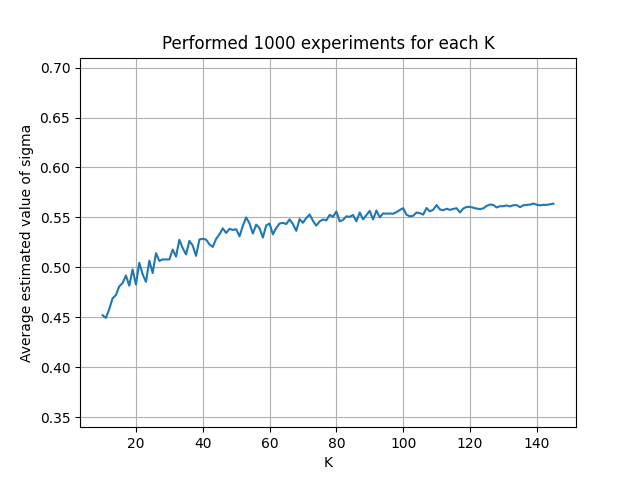
\includegraphics[width=\textwidth]{P1_sigma/avgs_1000.png}
        \caption[]{Average value of $\hat{\sigma}_{MLE}$ observed}
    \end{subfigure}
    \begin{subfigure}[H]{0.49\textwidth}
        \centering
        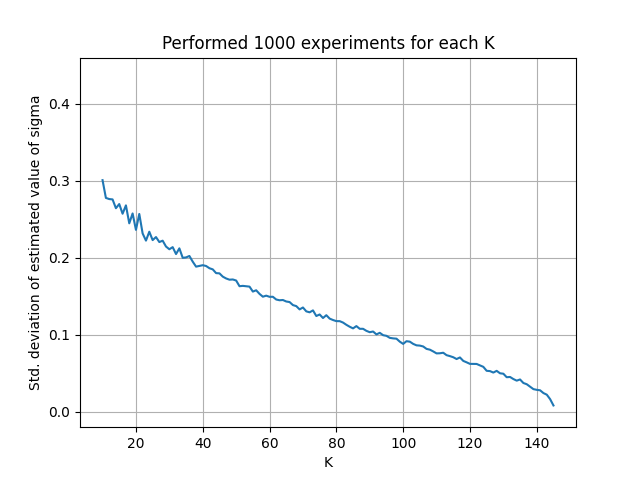
\includegraphics[width=\textwidth]{P1_sigma/stds_1000.png}
        \caption[]{Std. deviation of $\hat{\sigma}_{MLE}$ observed}
    \end{subfigure}
    \caption{Number of iterations, $N = 1000$}
\end{figure}

\subsection{Inference}
\begin{itemize}
    \item We can clearly observe that as $N$ increases, we are able to capture relation of variability of the estimates with $K$ very well.
    \item For large $N$, the expected value of estimate of $\mu$ for large $K$ is consistent (0.543).
    \item The expected value of estimate of $\sigma$ for large $N$ is dependent on $K$ because $\hat{\sigma^2}_{MLE}$ is proportional to a chi squared RV which has degrees of freedom dependent upon $K$.
    \item For small $N$, the average estimates for both $\mu$ and $\sigma$ vary more for small $K$. \\
          This can be explained by the large variance for small $K$.
\end{itemize}


\newpage
\section{Parameter estimation Problem 2}
\setcounter{figure}{0}
\subsection{Description}
The age of people who died in Greece in 2005 follows $\mathrm{Binomial}(p, 110)$. \\
We have age $a = (a_1, \cdots ,a_n)$ of people who died in Greece in 2005 given to us. \\
Estimated value of $p$ is $\hat{p}_{MLE} = \mathrm{mean}(a) / 110$.

\subsection{Experiment}
\verb!mortality_Country.csv! contains total deaths per age interval, we cannot generate $a$ directly. \\
We extract percentage of deaths in Greece in 2005 for each age interval. \\
We define a procedure which returns age of a person based on this percentage distribution. \\
We do this by using the CDF generated using the obtained percentage distribution and randomly sample real value in $[0, 1]$ and use this to get the age. \\
Using the above defined procedure, we generate a $K$ sized list of ages, and compute the estimate of $p$ ($\hat{p}_{MLE}$). We repeat this for $N$ iterations. \\
We intend to observe the variation in our estimate of $p$ for different $K$ and $N$.

\subsection{Results}
\begin{figure}[H]
    \centering
    \begin{subfigure}[H]{0.49\textwidth}
        \centering
        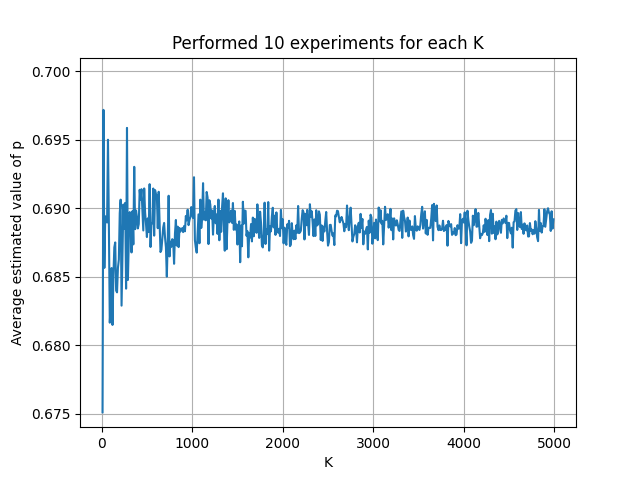
\includegraphics[width=\textwidth]{P2_p/avgs_10.png}
        \caption[]{Average value of $\hat{p}_{MLE}$ observed}
    \end{subfigure}
    \begin{subfigure}[H]{0.49\textwidth}
        \centering
        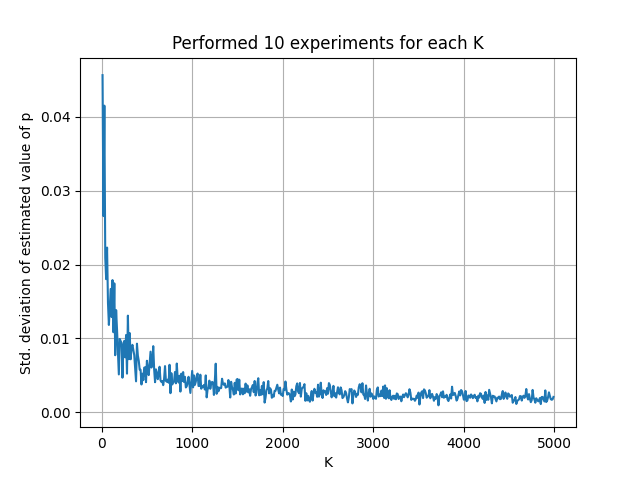
\includegraphics[width=\textwidth]{P2_p/stds_10.png}
        \caption[]{Std. deviation of $\hat{p}_{MLE}$ observed}
    \end{subfigure}
    \caption{Number of iterations, $N = 10$}
\end{figure}
\newpage
\begin{figure}[H]
    \centering
    \begin{subfigure}[H]{0.49\textwidth}
        \centering`
        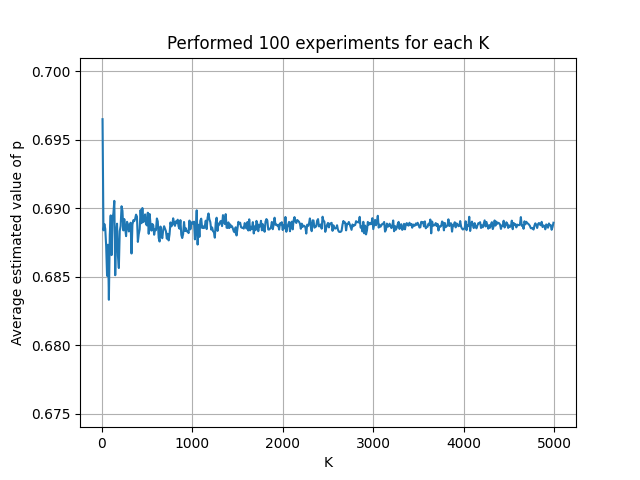
\includegraphics[width=\textwidth]{P2_p/avgs_100.png}
        \caption[]{Average value of $\hat{p}_{MLE}$ observed}
    \end{subfigure}
    \begin{subfigure}[H]{0.49\textwidth}
        \centering
        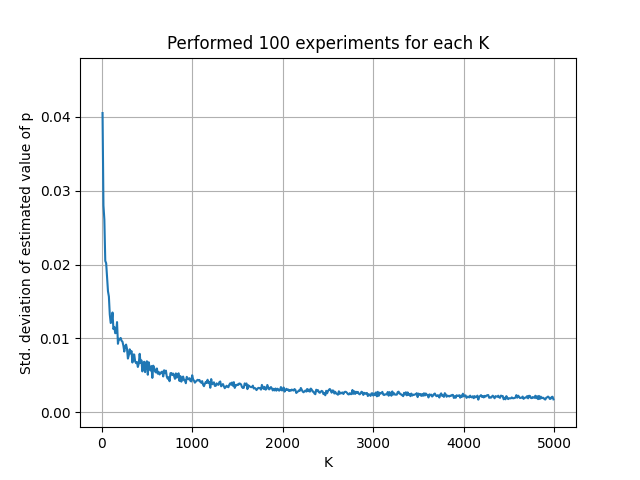
\includegraphics[width=\textwidth]{P2_p/stds_100.png}
        \caption[]{Std. deviation of $\hat{p}_{MLE}$ observed}
    \end{subfigure}
    \caption{Number of iterations, $N = 100$}
\end{figure}
\vspace{0pt}
\begin{figure}[H]
    \centering
    \begin{subfigure}[H]{0.49\textwidth}
        \centering
        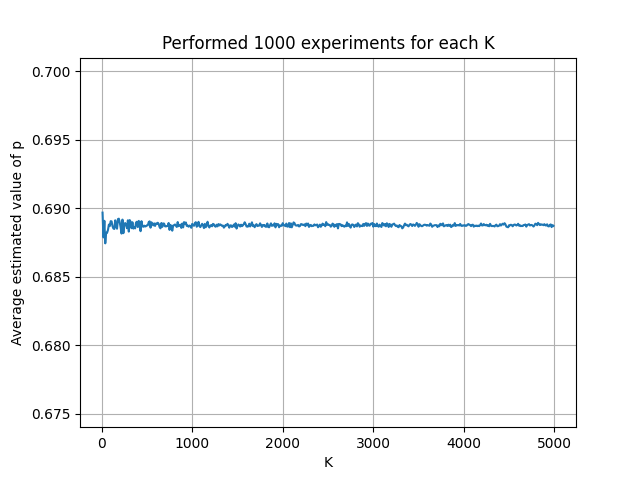
\includegraphics[width=\textwidth]{P2_p/avgs_1000.png}
        \caption[]{Average value of $\hat{p}_{MLE}$ observed}
    \end{subfigure}
    \begin{subfigure}[H]{0.49\textwidth}
        \centering
        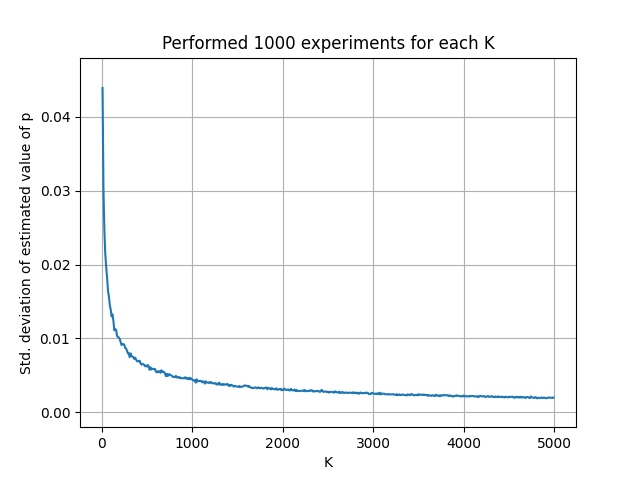
\includegraphics[width=\textwidth]{P2_p/stds_1000.png}
        \caption[]{Std. deviation of $\hat{p}_{MLE}$ observed}
    \end{subfigure}
    \caption{Number of iterations, $N = 1000$}
\end{figure}

\subsection{Inference}
\begin{itemize}
    \item We can clearly observe that as $N$ increases, we are able to capture relation of variability of the estimated value with $K$ very well.
    \item For large $N$, the expected value of estimate for all $K$ is consistent (almost 0.689). \\
          This sits well with law of large numbers.
    \item For small $N$, the average estimated varies more for small $K$. \\
          This can be explained by the large variance for small $K$.
\end{itemize}


\newpage
\section{Hypothesis Testing Problem 1}
\setcounter{figure}{0}
\subsection{Description}
We have two countries - Italy and Australia. \\
We have gender ratios $r = (r_1, \cdots ,r_n)$ of different years given to us for a specific country. \\
We observe that $r_i \sim \mathrm{Uniform}[\theta-\beta, \theta+\beta]$. \\
Given a sample, we hypothesise H0 (Null hypothesis) and H1 (Alternative hypothesis). \\
H0: Country is Italy \\
H1: Country is Australia \\
We perform following tests to accept/reject H0. \\
Test1: Reject H0 if $\mathrm{mean}(r) < 1.0$ \\
Test2: Reject H0 if $\hat{\theta}_{MLE} = \dfrac{\mathrm{max}(r) + \mathrm{min}(r)}{2} < 1.0$.

\subsection{Experiment}
From \verb!population_Country.csv!, we extract one unordered list of gender ratios for both countries. \\
The gender ratios are computed as ratio of total female population (using \verb!Female2! column) and total male population (using \verb!Male2! column) for every year. \\
The size of the unordered list is 147 for Italy and 98 for Australia. \\
We randomly choose a $K$ sized subset $(K \le 98)$ of one of the lists. We compare the output of both the tests with the true value. We repeat this for $2N$ iterations, where both countries have true value for $N$ iterations (to avoid dominance of either side of hypothesis). \\
We intend to observe the values of Type I error and Type II error for both the tests for different $K$ and $N$.

\subsection{Results}
\begin{figure}[H]
    \centering
    \begin{subfigure}[H]{0.49\textwidth}
        \centering
        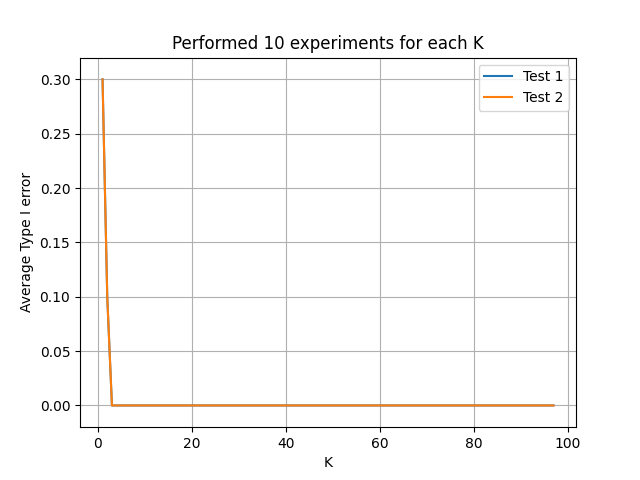
\includegraphics[width=\textwidth]{P3/type1_10.png}
        \caption[]{Average value of Type I error observed}
    \end{subfigure}
    \begin{subfigure}[H]{0.49\textwidth}
        \centering
        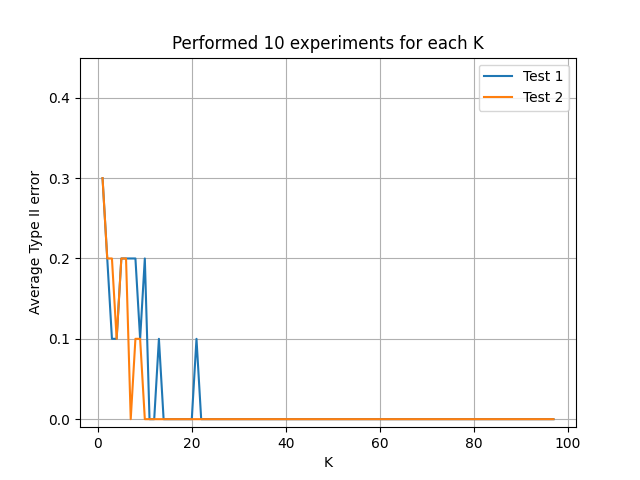
\includegraphics[width=\textwidth]{P3/type2_10.png}
        \caption[]{Average value of Type II error observed}
    \end{subfigure}
    \caption{Number of iterations for each side of hypothesis as truth, $N = 10$}
\end{figure}
\newpage
\begin{figure}[H]
    \centering
    \begin{subfigure}[H]{0.49\textwidth}
        \centering
        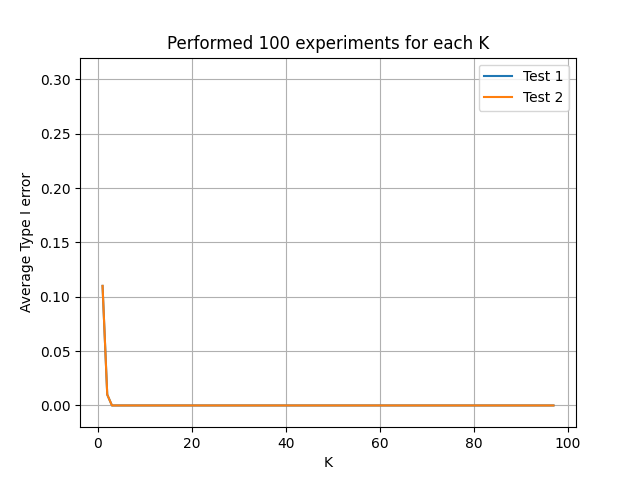
\includegraphics[width=\textwidth]{P3/type1_100.png}
        \caption[]{Average value of Type I error observed}
    \end{subfigure}
    \begin{subfigure}[H]{0.49\textwidth}
        \centering
        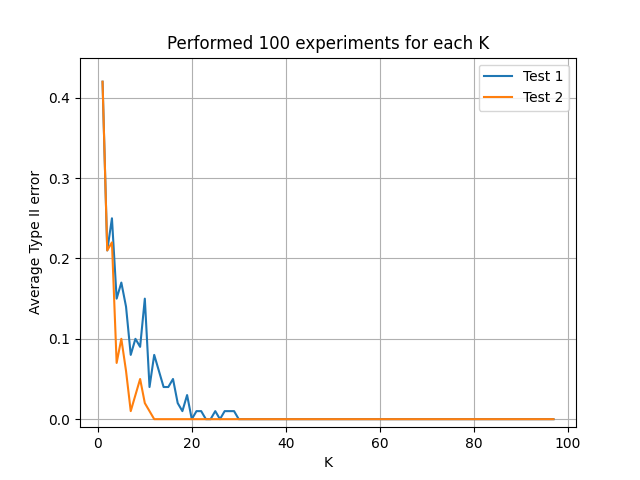
\includegraphics[width=\textwidth]{P3/type2_100.png}
        \caption[]{Average value of Type II error observed}
    \end{subfigure}
    \caption{Number of iterations for each side of hypothesis as truth, $N = 100$}
\end{figure}
\vspace{30pt}
\begin{figure}[H]
    \centering
    \begin{subfigure}[H]{0.49\textwidth}
        \centering
        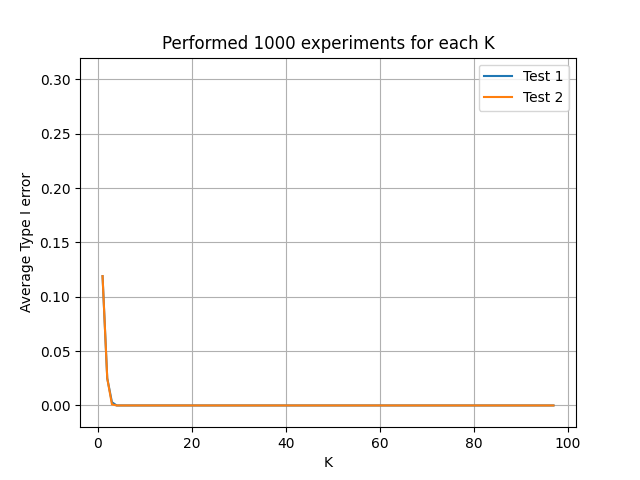
\includegraphics[width=\textwidth]{P3/type1_1000.png}
        \caption[]{Average value of Type I error observed}
    \end{subfigure}
    \begin{subfigure}[H]{0.49\textwidth}
        \centering
        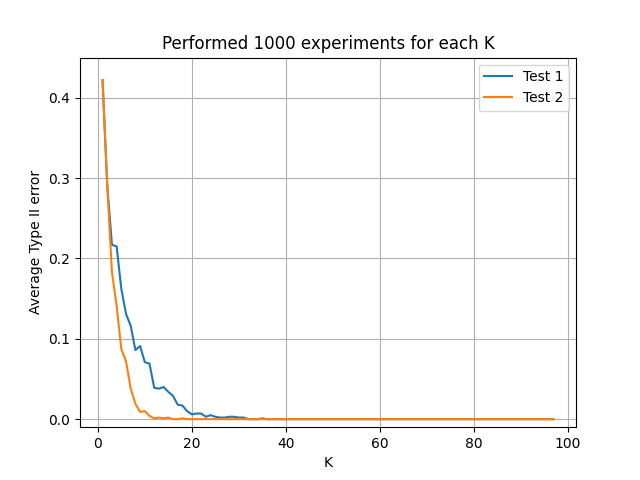
\includegraphics[width=\textwidth]{P3/type2_1000.png}
        \caption[]{Average value of Type II error observed}
    \end{subfigure}
    \caption{Number of iterations for each side of hypothesis as truth, $N = 1000$}
\end{figure}
\newpage
\begin{figure}[H]
    \centering
    \begin{subfigure}[H]{0.49\textwidth}
        \centering
        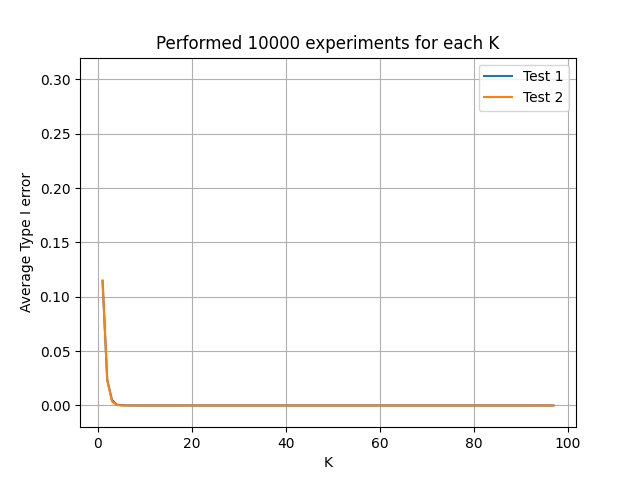
\includegraphics[width=\textwidth]{P3/type1_10000.png}
        \caption[]{Average value of Type I error observed}
    \end{subfigure}
    \begin{subfigure}[H]{0.49\textwidth}
        \centering
        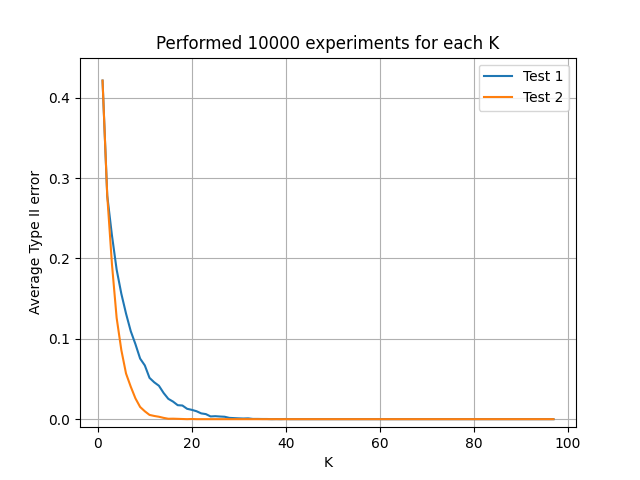
\includegraphics[width=\textwidth]{P3/type2_10000.png}
        \caption[]{Average value of Type II error observed}
    \end{subfigure}
    \caption{Number of iterations for each side of hypothesis as truth, $N = 10000$}
\end{figure}

\subsection{Inference}
\begin{itemize}
    \item As $N$ (i.e. the number of experiments for a given sample size) increases, we are able to capture relation of errors with $K$ (i.e the sample size) very well.
    \item The average value of Type I and Type II error for both tests decreases with the sample size for all values of N.
    \item Type I error is same for both tests. Type II error is less for Test 2. \\
          We can conclude that Test 2 is more powerful than Test 1.
\end{itemize}


\newpage
\section{Hypothesis Testing Problem 2}
\setcounter{figure}{0}
\subsection{Description}
We have two countries - Italy and Australia. \\
We have population growth rate $g = (g_1, \cdots ,g_n)$ of different years given to us for a specific country. \\
We observe that, if the ``specific country'' is Italy, $g_i \sim \mathcal{N}(\mu_1, \sigma_1^2)$; and if the ``specific country'' is Australia, $g_i \sim \mathcal{N}(\mu_2, \sigma_2^2)$. \\
Given a sample, we hypothesise H0 (Null hypothesis) and H1 (Alternative hypothesis). \\
H0: Country is Italy \\
H1: Country is Australia \\
We perform following test to accept/reject H0. \\
Test: Reject H0 if $\hat{\mu}_{MLE} = \mathrm{mean}(g) > 1.2$

\subsection{Experiment}
From \verb!population_Country.csv!, we determine population growth rate for both countries. \\
The population growth rates are computed as percentage change in population (using \verb!Total2! column) for every year. \\
The size of the list is 147 for Italy and 98 for Australia. \\
We randomly choose a $K$ sized subset $(K \le 98)$ from one of the lists. We compare the output of the test with the true value. We repeat this for $2N$ iterations, where both countries have true value for $N$ iterations (to avoid dominance of either side of hypothesis). \\
We intend to observe the values of Type I error and Type II error for the test for different $K$ and $N$.

\subsection{Results}
\begin{figure}[H]
    \centering
    \begin{subfigure}[H]{0.49\textwidth}
        \centering
        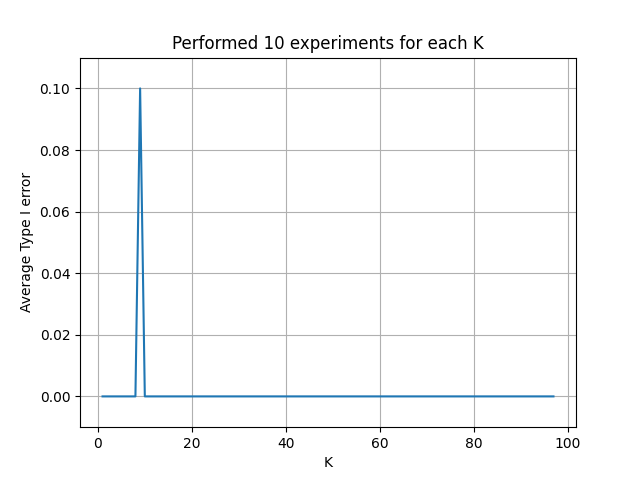
\includegraphics[width=\textwidth]{P4/type1_10.png}
        \caption[]{Average value of Type I error observed}
    \end{subfigure}
    \begin{subfigure}[H]{0.49\textwidth}
        \centering
        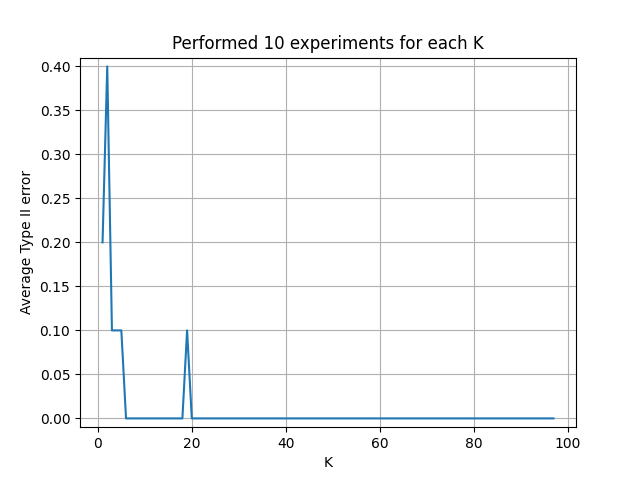
\includegraphics[width=\textwidth]{P4/type2_10.png}
        \caption[]{Average value of Type II error observed}
    \end{subfigure}
    \caption{Number of iterations for each side of hypothesis as truth, $N = 10$}
\end{figure}
\newpage
\begin{figure}[H]
    \centering
    \begin{subfigure}[H]{0.49\textwidth}
        \centering
        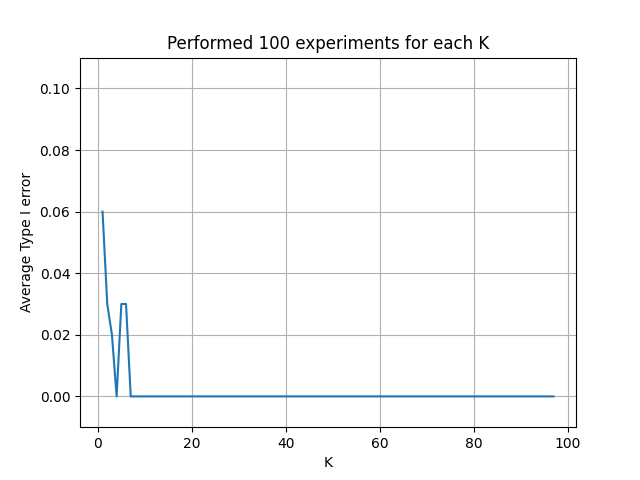
\includegraphics[width=\textwidth]{P4/type1_100.png}
        \caption[]{Average value of Type I error observed}
    \end{subfigure}
    \begin{subfigure}[H]{0.49\textwidth}
        \centering
        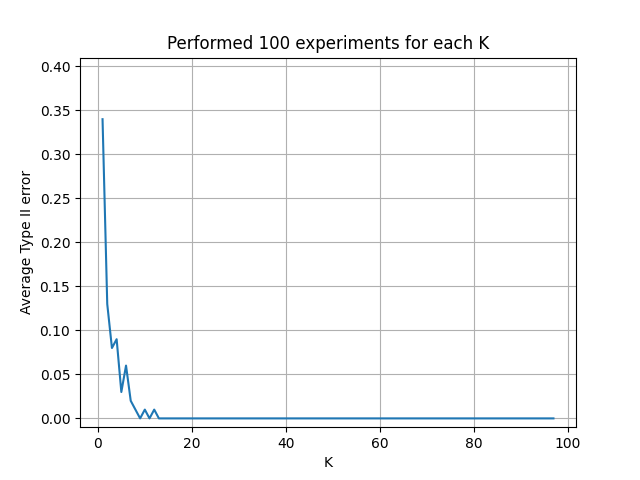
\includegraphics[width=\textwidth]{P4/type2_100.png}
        \caption[]{Average value of Type II error observed}
    \end{subfigure}
    \caption{Number of iterations for each side of hypothesis as truth, $N = 100$}
\end{figure}
\vspace{30pt}
\begin{figure}[H]
    \centering
    \begin{subfigure}[H]{0.49\textwidth}
        \centering
        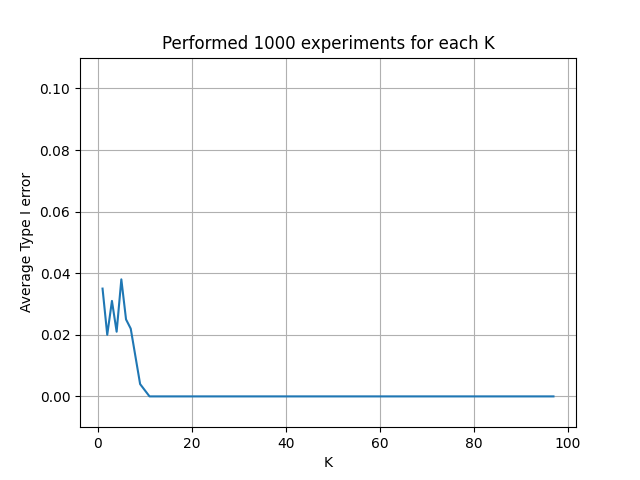
\includegraphics[width=\textwidth]{P4/type1_1000.png}
        \caption[]{Average value of Type I error observed}
    \end{subfigure}
    \begin{subfigure}[H]{0.49\textwidth}
        \centering
        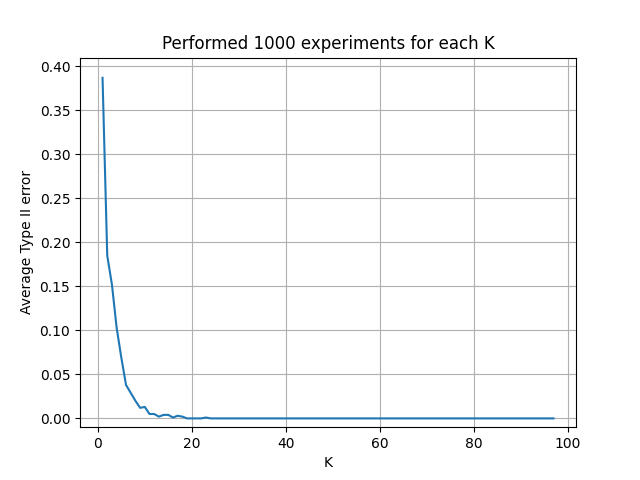
\includegraphics[width=\textwidth]{P4/type2_1000.png}
        \caption[]{Average value of Type II error observed}
    \end{subfigure}
    \caption{Number of iterations for each side of hypothesis as truth, $N = 1000$}
\end{figure}
\newpage
\begin{figure}[H]
    \centering
    \begin{subfigure}[H]{0.49\textwidth}
        \centering
        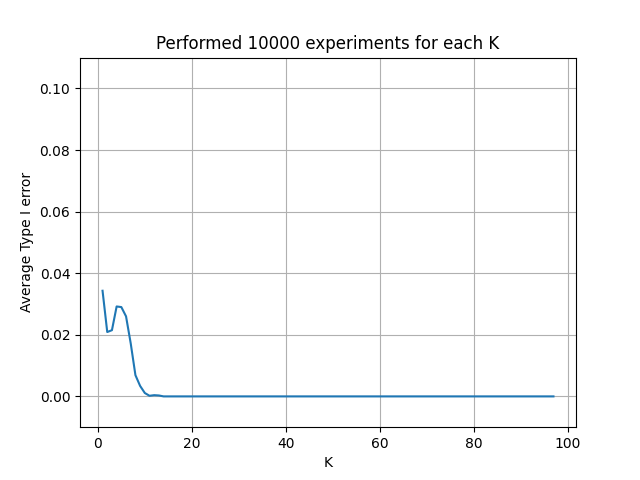
\includegraphics[width=\textwidth]{P4/type1_10000.png}
        \caption[]{Average value of Type I error observed}
    \end{subfigure}
    \begin{subfigure}[H]{0.49\textwidth}
        \centering
        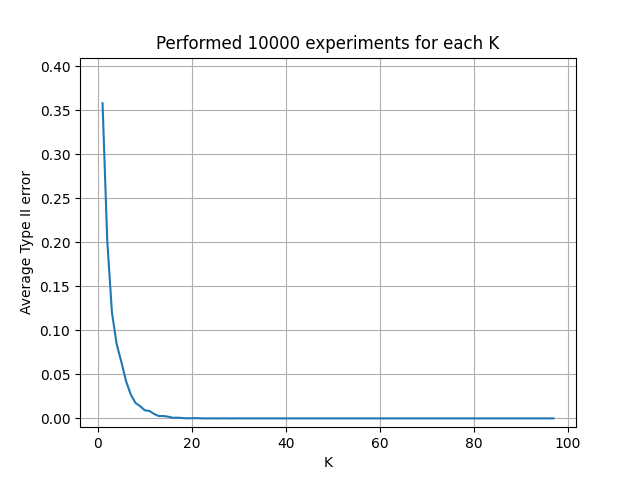
\includegraphics[width=\textwidth]{P4/type2_10000.png}
        \caption[]{Average value of Type II error observed}
    \end{subfigure}
    \caption{Number of iterations for each side of hypothesis as truth, $N = 10000$}
\end{figure}

\subsection{Inference}
\begin{itemize}
    \item As $N$ (i.e. the number of experiments for a given sample size) increases, we are able to capture relation of errors with $K$ (i.e the sample size) very well.
    \item The average value of Type I and Type II error decreases with the sample size for all values of N.
    \item The Type II error is more prevalent (i.e. has a higher probability of occurrence) for small values of $K$. At larger $K$ values, both errors are practically zero.
\end{itemize}



\end{document}
